\providecommand{\main}{..}
\documentclass[\main/master.tex]{subfiles}
\begin{document}
\section{garvity measurement past results}
\chapter{introduction}\label{chp:example-1}
\doublespacing
\hspace{5 mm} This is a \LaTeX template for preparing a dissertation according to the University of Rochester guidelines \cite{uofr_guidelines} as of July 2020. It also includes some useful \LaTeX formatting including a working example of a bibliography. You will need a working TeX distribution such as MikTeX \cite{miktex_home} or TeXLive \cite{texlive_nodate} to compile this document.  \par
Here is an example equation (from \cite{einstein1905tragheit}) that has it's own label we will reference in Chapter~\ref{chp:example-2}:
\begin{equation}
E=mc^{2}.\label{eqn:energy-mass-equivalence-relation}
\end{equation}
Here is an example image:
\begin{figure}[htbp]
	\centering
	\fbox{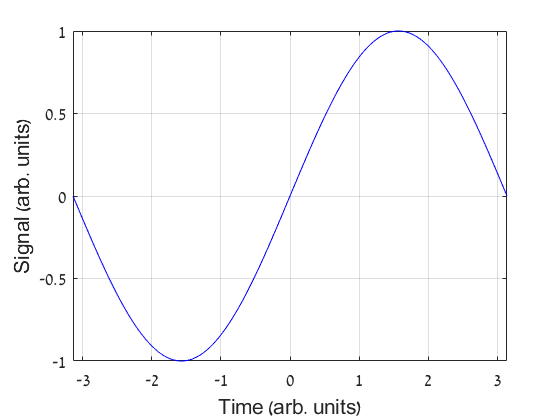
\includegraphics[scale=0.5]{\main/images/chapter_1_example/img_example.png}}
	\caption[Example Image]{Example Image. This image is also labeled internally so we can reference it throughout the text.}
	\label{fig:sine-wave}
\end{figure}
If you want to reference the example figure (Fig.~\ref{fig:sine-wave}), you can. See also Fig.~\ref{fig:cosine-wave}.


\end{document}